
\section{来自射影几何的重要例子}

我们现在要用\trGradedRing{}的语言来解读\trClosedEmbedding。不必担心：分次环那套烦人的基础性讨论大都已告完成，如今我们只管坐享先前工作的成果。

\textbf{9.3.1.\ 例：射影空间 $\mathbb{P}^n_A$ 中的\trClosedEmbedding。}\quad 回想\cref{thm:projective-space-over-ring}中给出的 $\mathbb{P}^n_A$ 的定义（以及其中定义的术语）。$x_0,\dots,x_n$ 的任何\trHomogeneous{}多项式 $f$ 都定义了一个\trClosedSubscheme。（因此，即便 $f$ 作为函数没有意义，它的\trVanishingScheme{}仍有意义。）在\trOpenSet{} $U_i$ 上，这个\trClosedSubscheme{}是 $V(f(x_{0/i},\dots,x_{n/i}))$，我们私下里把它想作 $V(f(x_0,\dots,x_n)/x_i^{\deg f})$。在交叠处
\[
U_i\cap U_j=\Spec A[x_{0/i},\dots,x_{n/i},x_{j/i}^{-1}]/(x_{i/i}-1)
\]
上，$U_i$ 与 $U_j$ 上的这两个函数并不完全一致，但至多相差一个不消失的标量，因此切出 $U_i\cap U_j$ 的同一个\trClosedSubscheme（\cref{ex:vanishing-scheme-global-section}(b)）：
\[
f(x_{0/i},\dots,x_{n/i})=x_{j/i}^{\deg f}f(x_{0/j},\dots,x_{n/j}).
\]
类似地，$A[x_0,\dots,x_n]$ 中的一组\trHomogeneous{}多项式切出 $\mathbb{P}^n_A$ 的一个\trClosedSubscheme。（\mbox{练习~15.7.I} 将证明：$\mathbb{P}^n_A$ 的一切\trClosedSubscheme{}都具有这种形式。）

\textbf{9.3.2.}\ \emph{\trhDefinition{}。}\quad 照例，设 $k$ 是一个\trField。$\mathbb{P}^n_k$ 中由单个（非零、\trHomogeneous{}的）方程切出的\trClosedSubscheme{}称为一个\textbf{\trHypersurface}（在 $\mathbb{P}^n_k$ 中）。（小心：「超曲面」一词在代数几何中可以指略有不同的东西，而且各有全然合理的缘由；例如见 \S12.1.5。）当然，超曲面并不是由 $\mathbb{P}^n_k$ 上的单个整体函数切出的：非常值的整体函数根本不存在（\cref{ex:proj-functions-constant}）。超曲面的\trDegree{}就是那个多项式的次数。（这话里暗含着一层意思：这个观念可以从子概形自身定出来。你现在或许已手握证明它的工具，但我们要到\mbox{练习~18.6.G}才正式证明它。）次数 $1$（相应地，次数 $2$、$3$、……）的超曲面称为\trHyperplane{}（相应地，\textbf{二次}（quadric）、\textbf{三次}（cubic）、\textbf{四次}（quartic）、\textbf{五次}（quintic）、\textbf{六次}（sextic）、\textbf{七次}（septic）、\textbf{八次}（octic）、……超曲面）。当 $n=2$ 时，超曲面称为\trCurve；次数 $1$ 的超曲面称为直线，而次数 $2$ 的超曲面称为\trConic{}（conic curve），或简称\trConic。当 $n=3$ 时，超曲面称为\trSurface。（在第 12 章中，我们将为曲线与曲面这两个名号正名。）

\textbf{9.3.A.（练习）}\quad
\begin{enumerate}[label=(\alph*)]
  \item 证明：$wz=xy$、$x^2=wy$、$y^2=xz$ 描述了 $\mathbb{P}^3_k$ 中一个\trIrreducible{}的\trClosedSubscheme。事实上它是一条\trCurve——这个观念要等我们知道了\trDimension{}为何物之后才来定义。这条曲线称为\textbf{\trTwistedCubic{}}（twisted cubic）。（\trTwistedCubic{}是许多事物的绝佳非平凡例子，所以你应当尽早跟它交上朋友。它在前面的\cref{ex:twisted-cubic-cone}中已隐然登场。）
  \item 证明：\trTwistedCubic{}\trIsomorphic{}于 $\mathbb{P}^1_k$。
\end{enumerate}

现在我们把这一讨论推广到一般的\trProjectiveScheme。

\textbf{9.3.B.（练习）}\quad 设 $S_\bullet\twoheadrightarrow R_\bullet$ 是\trGradedRing{}之间的一个满射。证明：由之诱导的\trMorphism（\mbox{练习~7.4.A}）的定义域是 $\Proj R_\bullet$，并且所诱导的\trMorphism{} $\Proj R_\bullet\to\Proj S_\bullet$ 是一个\trClosedEmbedding。

\mbox{练习~15.7.I} 将证明\mbox{练习~9.3.B}的逆命题：射影 $A$-\trScheme{}中的每个\trClosedEmbedding{} $X\hookrightarrow\Proj S_\bullet$（$S_\bullet$ 是一个有限生成的\trGrading{} $A$-\trAlgebra）都形如 $\Proj(S_\bullet/I)$，其中 $I$ 是一个\trHomogeneous\trIdeal，由在 $X$ 上消失的「射影函数」组成。（你现在或许就有本事证明这一点。）

\textbf{9.3.C.（练习）}\quad 证明：$k$-\trVectorSpace{}之间的一个单的线性映射 $V\hookrightarrow W$ 诱导一个\trClosedEmbedding{} $\mathbb{P}V\hookrightarrow\mathbb{P}W$。（这是对\mbox{例~4.5.13}中用 $V$ 的\trDual{}来定义 $\mathbb{P}V$ 的又一次辩护。）

\textbf{9.3.3.}\ \emph{\trhDefinition{}。}\quad \mbox{练习~9.3.C}中定义的那个\trClosedSubscheme{}称为一个\textbf{\trLinearSpace{}}（linear space）。等我们懂得\trDimension{}之后，将把这个\trClosedSubscheme{}称为维数 $\dim V-1=\dim\mathbb{P}V$ 的\trLinearSpace{}。更显式地说，$\mathbb{P}^N$ 中维数 $n$ 的\trLinearSpace{}，就是由 $x_0,\dots,x_N$ 中 $N-n$ 个 $k$-线性无关的\trHomogeneous{}线性多项式切出的任何\trClosedSubscheme。维数 $1$（相应地，$2$、$n$、$\dim\mathbb{P}V-1$）的\trLinearSpace{}称为直线（相应地，平面、$n$-平面、\trHyperplane）。（若上一道练习中的线性映射不单，则\mbox{练习~7.4.A}的假设 \eqref{eq:vphi-s-plus-empty} 便不成立。）

\textbf{9.3.D.（练习：\trBezout{}（Bézout）定理的一个特殊情形）}\quad 设 $X\subset\mathbb{P}^n_k$ 是由 $f=0$ 切出的一张次数 $d$ 的超曲面，而 $\ell$ 是一条不含于 $X$ 的直线。\trBezout{}定理（\mbox{练习~18.6.J}）的一个非常特殊的情形蕴含：$X$ 与 $\ell$ 以重数 $d$ 相交（「按正确的方式计数」）。请把这件事说出个道理来：把齐次的次数 $d$ 多项式 $f$ 限制到直线 $\ell$ 上，并利用「$k[x]$ 中次数 $d$ 的多项式有 $d$ 个根（按妥当的方式计数）」这一事实。（如果你觉得这样心里更踏实，不妨假定 $k=\overline{k}$。）

\textbf{9.3.E.（练习）}\quad 证明：由 $(w,x,y,z)\mapsto(s^3,s^2t,st^2,t^3)$ 给出的\trGradedRing{}的\trMap{} $k[w,x,y,z]\to k[s,t]$ 诱导一个\trClosedEmbedding{} $\mathbb{P}^1_k\hookrightarrow\mathbb{P}^3_k$，而它给出 $\mathbb{P}^1_k$ 与\trTwistedCubic{}（定义于\mbox{练习~9.3.A}——事实上，这将顺带解出\mbox{练习~9.3.A}(b)）的一个\trIsomorphism。亲手做一遍这件事，会为你应对 \S9.3.6 的一般\trVeronese{}构造打下很好的底子；推广见\mbox{练习~9.3.I}。

\textbf{9.3.4.\ 一个特别好的情形：$S_\bullet$ 在次数 $1$ 处生成。}\quad 设 $S_\bullet$ 是一个在次数 $1$ 处生成的\trFinitelyGenerated\trGradedRing。那么 $S_1$ 是一个有限生成的 $S_0$-\trModule，而\trIrrelevantIdeal{} $S_+$ 在次数 $1$ 处生成（参\cref{ex:fg-graded-rings}(a)）。

\textbf{9.3.F.（练习）}\quad 证明：若 $S_\bullet$ 作为 $A$-\trAlgebra{}在次数 $1$ 处由 $n+1$ 个元素 $x_0,\dots,x_n$ 生成，则 $\Proj S_\bullet$ 可以按如下方式描述为 $\mathbb{P}^n_A$ 的一个\trClosedSubscheme。把 $A^{\oplus(n+1)}$ 看作一个\trFreeModule，它带有一组\trGenerator{} $t_0,\dots,t_n$，依次关联于 $x_0,\dots,x_n$。于是，满射
\[
\begin{gathered}
\Sym^{\bullet}\bigl(A^{\oplus(n+1)}\bigr)=A[t_0,t_1,\dots,t_n]\twoheadrightarrow S_\bullet,\\
t_i\longmapsto x_i,
\end{gathered}
\]
蕴含 $S_\bullet=A[t_0,t_1,\dots,t_n]/I$，其中 $I$ 是一个\trHomogeneous\trIdeal。（特别地，只要 $S_\bullet$ 在次数 $1$ 处有限生成，$\Proj S_\bullet$ 就总能被解读为某个 $\mathbb{P}^n_A$ 的\trClosedSubscheme。而后，借助\mbox{练习~7.4.D}与\mbox{练习~7.4.G}，你还可以把「在次数 $1$ 处生成」这一假设去掉。）

这与下述事实类似：若 $R$ 是一个有限生成的 $A$-\trAlgebra，则作为代数选取 $R$ 的 $n$ 个\trGenerator，就等价于把 $\Spec R$ 描述为 $\mathbb{A}^n_A$ 的一个\trClosedSubscheme。在仿射的情形，这叫作「选取\trCoordinate」；在射影的情形，这叫作「选取\trProjective\trCoordinate」。

回想（\cref{ex:closed-points-pn-traditional}）：若 $k$ \trAlgClosed，则我们可以把 $\mathbb{P}^n$ 的\trClosedPoint{}解读为 $(n+1)$ 维空间中过原点的诸直线。下面的练习把这件事陈述得更为一般。

\textbf{9.3.G.（练习）}\quad 设 $S_\bullet$ 是\trAlgClosedField{} $k$ 上一个有限生成的\trGradedRing，在次数 $1$ 处由 $x_0,\dots,x_n$ 生成，从而诱导闭嵌入 $\Proj S_\bullet\hookrightarrow\mathbb{P}^n$ 与 $\Spec S_\bullet\hookrightarrow\mathbb{A}^{n+1}$。请在 $\Proj S_\bullet$ 的诸\trClosedPoint{}与 $\Spec S_\bullet\subset\mathbb{A}^{n+1}$ 中「过原点的直线」之间给出一个\trBijection。

\textbf{9.3.5.}\ \emph{有限\trMorphism{}为闭的第二个证明。}\quad 把 $\Proj S_\bullet$ 解读为\trProjectiveSpace{}的\trClosedSubscheme（当它在次数 $1$ 处生成时），便给出下述第二个证明：有限\trMorphism{}是闭的（\mbox{练习~8.3.L}中已证）。设 $\pi\colon X\to Y$ 是一个\trFinite\trMorphism。这个问题对目标是局部的，故不妨考虑仿射情形 $Y=\Spec B$。只需证明 $\pi(X)$ 是闭的。于是由\mbox{练习~8.3.I}，$X$ 是一个\trProjective{}的 $B$-\trScheme，从而由\trFundamentalTheoremOfEliminationTheory{}~8.4.10，它的像是闭的。

\textbf{9.3.6.\ 重要的经典构造：\trVeroneseEmbedding。}\quad 设 $S_\bullet=k[x,y]$，于是 $\Proj S_\bullet=\mathbb{P}^1_k$。那么 $S_{2\bullet}=k[x^2,xy,y^2]\subset k[x,y]$（关于\trVeroneseSubring，见 \S7.4.4）。我们按如下方式认出这个子环。

\textbf{9.3.H.（练习）}\quad 令 $u=x^2$、$v=xy$、$w=y^2$。证明：把 $u$、$v$、$w$ 分别映到 $x^2$、$xy$、$y^2$，便有 $S_{2\bullet}\cong k[u,v,w]/(uw-v^2)$。

我们得到一个由三个元素在次数 $1$ 处生成的\trGradedRing。于是，经由\mbox{练习~9.3.F}的构造，我们把它想作「坐」在 $\mathbb{P}^2$ 里。这可以被解读为「作为 $\mathbb{P}^2$ 中一条\trConic{}的 $\mathbb{P}^1$」。

\textbf{9.3.7.}\quad 于是，若 $k$ 是\trCharacteristic{}不为 $2$ 的\trAlgClosedField，利用「二次型可以对角化」（\mbox{练习~5.4.J}）这一事实，$\mathbb{P}^2$ 中的诸\trConic{}在换坐标的意义下只有寥寥数种风味：三个（且无法更少）平方数之和（例如上一道练习中的那张\trConic）、两个（且无法更少）平方数之和（例如 $y^2-x^2=0$，即两条直线之并）、单个（非零）平方（例如 $x^2=0$，它在集合的层面上看似一条直线，且非\trReduced），以及 $0$（或许压根算不上\trConic）。于是我们便证明了：任何平面\trConic（在\trCharacteristic{}不为 $2$ 的\trAlgClosedField{}上），只要能写成三个非零平方数之和（且无法更少），就\trIsomorphic{}于 $\mathbb{P}^1$。（与此密切相关的一个事实，见\mbox{练习~7.5.G}。）

我们现在来把这个例子升级改装一番。

\textbf{9.3.I.（练习）}\quad 我们继续取 $S_\bullet=k[x,y]$。证明：$\Proj S_{d\bullet}$ 由「下述矩阵的\trRank{}为 $1$」这组方程给出（也就是说，由「一切 $2\times2$ \trMinor{}（minor）都为零」给出）：
\[
\begin{pmatrix}
y_0 & y_1 & \cdots & y_{d-1}\\
y_1 & y_2 & \cdots & y_d
\end{pmatrix}
\]
它称为「居于」$\mathbb{P}^d$ 中的\textbf{次数 $d$ \trRationalNormalCurve{}}（degree $d$ rational normal curve）。$d=3$ 的\trTwistedCubic{}情形你已在\mbox{练习~9.3.A}与\mbox{练习~9.3.E}中做过。

\textbf{9.3.8.}\ \emph{\trhDefinition{}。}\quad 更一般地，若 $S_\bullet=k[x_0,\dots,x_n]$，则映射 $\nu_d\colon\Proj S_{d\bullet}\to\mathbb{P}^{N-1}$（其中 $N$ 是 $x_0,\dots,x_n$ 的齐次次数 $d$ 多项式所构成的\trVectorSpace{}的\trDimension）称为\textbf{$d$ 重嵌入}（d-uple embedding），或（$d$ 重）\textbf{\trVeroneseEmbedding}。（把\mbox{练习~7.4.E}与\mbox{练习~9.3.F}结合起来便知 $\nu_d$ 是一个\trClosedEmbedding。）

\textbf{9.3.J.（组合练习；参看注记~4.5.3）}\quad 证明：$N=\binom{n+d}{d}$。

\textbf{9.3.K.（不重要练习）}\quad 找出六个线性无关的、在\trVeronese{}曲面 $\Proj S_{2\bullet}$ 上为零的二次方程，其中 $S_\bullet=k[x_0,x_1,x_2]$，而该曲面自然地居于 $\mathbb{P}^5$ 中。（你无须证明这些方程生成切出该\trVeronese{}曲面的全部方程，尽管这事实上为真。）可能的提示：使用恒等式
\[
\det\begin{pmatrix}
x_0x_0 & x_0x_1 & x_0x_2\\
x_1x_0 & x_1x_1 & x_1x_2\\
x_2x_0 & x_2x_1 & x_2x_2
\end{pmatrix}=0.
\]

\textbf{9.3.9.\ 二次曲面上的\trRuling。}\quad 我们回到二次曲面上的\trRuling{}这一话题；它最初出现在选学的（带星标的）\cref{thm:quadric-cone-section-example}中。

\textbf{9.3.L.（有用的几何练习：二次曲面 $wz=xy$ 上的\trRuling）}\quad 这道练习关乎 $\mathbb{P}^3_k$ 中由 $wz-xy=0$ 给出的二次曲面 $X$ 上的诸直线（其中 $\mathbb{P}^3_k$ 的\trProjective\trCoordinate{}按 $w$、$x$、$y$、$z$ 的次序排列）。这一构造在自然界里随处都会冒出来。
\begin{enumerate}[label=(\alph*)]
  \item 设 $a_0$ 与 $b_0$ 是 $k$ 中给定的两个元素，不全为零。请把下面这句话说出个道理来：当 $[c,d]$ 在 $\mathbb{P}^1$ 中变动时，$[a_0c,\,b_0c,\,a_0d,\,b_0d]$ 是该二次曲面中的一条直线。（这描述了「由 $\mathbb{P}^1$ 参数化的一族直线」，尽管我们还无法把这句话说精确。）再找出另一族直线。这两族便是光滑二次曲面的两族\trRuling。
  \item 证明：过二次曲面 $X$ 的每个 $k$-\trValuedPoint，两族\trRuling{}中各有一条直线经过。
  \item 证明：除此以外再无其他直线。（可行的做法很多。冒着让你先入为主的风险，这里给出一粒想法的「芽」。\footnote{译注：原文 \emph{germ of an idea} 一语双关——germ 既指「萌芽的想法」，也是本书中的术语「芽」。}设 $L$ 是二次曲面上的一条直线，而 $[1,x,y,z]$ 与 $[1,x',y',z']$ 是它上面两个不同的点。由于二者都落在二次曲面上，有 $z=xy$ 与 $z'=x'y'$。又由于 $L$ 整条落在二次曲面上，对一切 $t$ 都有 $(1+t)(z+tz')-(x+tx')(y+ty')=0$。经过一些代数变形，这就化为 $(x-x')(y-y')=0$。怎样才能把这一论证做得滴水不漏？另一种可能的做法是诉诸\trBezout{}定理（以\mbox{练习~9.3.D}的形式）。）
\end{enumerate}

\begin{figure}[htbp]
\centering
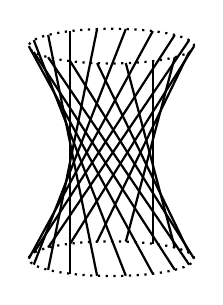
\begin{tikzpicture}[scale=1.0,line width=0.8pt]
  \draw[dotted] (0,1.35) ellipse (1.05 and 0.22);
  \draw[dotted] (0,-1.35) ellipse (1.05 and 0.22);
  \foreach \t in {0,20,...,340}
    \draw ({1.05*cos(\t)},{1.35+0.22*sin(\t)}) -- ({1.05*cos(\t+120)},{-1.35+0.22*sin(\t+120)});
\end{tikzpicture}
\caption{二次曲面 $S:=V(wz-xy)\subset\mathbb{P}^3$ 的两族\trRuling{}之一。一族\trRuling{}含有直线 $V(w,x)$，另一族则含有直线 $V(w,y)$。（图中草绘的这张二次曲面其实是 $a^2+b^2=c^2+1$。你能看出为什么它是 $S$ 的一个\trAffine\trCoordinatePatch{}吗？用 $w$、$x$、$y$、$z$ 来表示，$a$、$b$、$c$ 各是什么？提示：\mbox{练习~5.4.J}。）（依原书手绘图重绘。）}\label{fig:ruling-quadric-surface}
\end{figure}

于是，借助\mbox{练习~5.4.J}，若我们在\trCharacteristic{}不为 $2$ 的\trAlgClosedField{}上工作，我们便已证明：一切秩为 $4$ 的二次曲面都有两族由直线组成的\trRuling。（在\mbox{例~10.6.2}中，我们将认出这个二次曲面就是 $\mathbb{P}^1\times\mathbb{P}^1$。）

\textbf{9.3.10.}\ \emph{旁注：二次超曲面上的\trRuling。}\quad 这两族\trRuling{}的存在性，是好几个重要而美妙的故事共同的第一章。第二章则往往是下面这个。若 $k$ 是\trAlgClosedField，则维数 $m$ 的极大秩（\mbox{练习~5.4.J}）二次超曲面 $X$ 不含维数大于 $m/2$ 的\trLinearSpace{}。（我们将在\mbox{练习~13.3.D}中看到：极大秩的二次超曲面正是「光滑的」二次超曲面。）若 $m=2a+1$，则 $X$ 含有一个不可约的 $\binom{a+2}{2}$ 维的 $a$-平面族。若 $m=2a$，则 $X$ 含有两个不可约的 $\binom{a+1}{2}$ 维的 $a$-平面族；而且，两个 $a$-平面 $\Lambda$ 与 $\Lambda'$ 属于同一族，当且仅当 $\dim(\Lambda\cap\Lambda')\equiv a\pmod 2$。这些\trLinearSpace{}族也称为\trRuling。（欲知更多，可参 [GH1, \S6.1, p.~735, Prop.]。以你现有的知识，已足以想通 $m=0$、$1$、$2$ 的那些例子。$m=2$ 的情形——二次曲面上的\trRuling——将出现在\cref{thm:quadric-cone-section-example}、图~\ref{fig:ruling-quadric-surface}、\mbox{练习~9.3.L}、\S10.6.2、\S12.2.19、\S13.2.12、\mbox{练习~15.5.Q}与\mbox{练习~19.10.M}之中。$m=3$ 的情形则在\mbox{练习~16.4.K}中讨论。）

\textbf{9.3.11.\ \trAffine\trCone{}与\trProjective\trCone{}（图~\ref{fig:cones-of-proj}）。}\quad 若 $S_\bullet$ 是一个\trFinitelyGenerated\trGradedRing，则 $\Proj S_\bullet$ 的\trAffine\trCone{}是 $\Spec S_\bullet$。（警告：这一术语并不理想，因为这个构造依赖于 $S_\bullet$，而不只依赖于 $\Proj S_\bullet$。）作为动机，考察分次环 $S_\bullet=\mathbb{C}[x,y,z]/(z^2-x^2-y^2)$。图~\ref{fig:traditional-cone}是 $\Spec S_\bullet$ 的一幅草图。（这里我们画的是 $z^2=x^2+y^2$ 在 $\mathbb{R}^3$ 中的「实图像」。）它是传统意义上的一个\trCone；原点 $(0,0,0)$ 便是「锥点」。

这给出了一种设想 $\Proj$ 的有用方式（甚至在任意\trRing{}上都行，不限于 $\mathbb{C}$）。直观上，你可以想象：若把原点扔掉，得到的东西便可以投射到 $\Proj S_\bullet$ 上。下面的练习将把这件事说精确。

\begin{figure}[htbp]
\centering
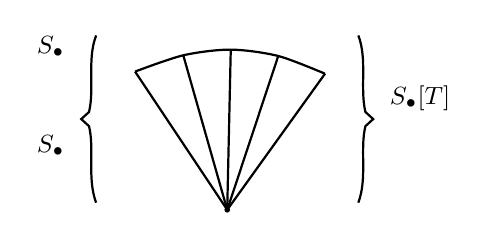
\begin{tikzpicture}[scale=0.9,line width=0.8pt,every node/.style={font=\small}]
  \fill (0,0) circle (0.04);
  \draw plot [smooth] coordinates {(-1.30,1.95) (-0.62,2.18) (0.05,2.26) (0.72,2.17) (1.38,1.92)};
  \draw (0,0) -- (-1.30,1.95);
  \draw (0,0) -- (-0.62,2.18);
  \draw (0,0) -- (0.05,2.26);
  \draw (0,0) -- (0.72,2.17);
  \draw (0,0) -- (1.38,1.92);
  \draw
    (-1.85,0.10)
    .. controls (-1.98,0.45) and (-1.87,0.85) .. (-1.95,1.18)
    -- (-2.06,1.28) -- (-1.95,1.38)
    .. controls (-1.87,1.72) and (-1.98,2.12) .. (-1.85,2.46);
  \draw
    (1.85,0.10)
    .. controls (1.98,0.45) and (1.87,0.85) .. (1.95,1.18)
    -- (2.06,1.28) -- (1.95,1.38)
    .. controls (1.87,1.72) and (1.98,2.12) .. (1.85,2.46);
  \node[anchor=east] at (-2.15,2.30) {$\Proj S_\bullet$};
  \node[anchor=east,align=right] at (-2.15,1.00) {\trAffine\trCone\\ $\Spec S_\bullet$};
  \node[anchor=west,align=left] at (2.15,1.65) {\trProjective\trCone\\ $\Proj S_\bullet[T]$};
\end{tikzpicture}
\caption{$\Proj S_\bullet$ 的\trAffine\trCone{}与\trProjective\trCone{}。（依原书手绘图重绘。）}\label{fig:cones-of-proj}
\end{figure}

\textbf{9.3.M.（练习）}\quad 若 $\Proj S_\bullet$ 是\trField{} $k$ 上的一个\trProjectiveScheme，请描述一个自然的\trMorphism{} $\Spec S_\bullet\setminus V(S_+)\to\Proj S_\bullet$。（你能看出为什么 $V(S_+)$ 恰是一个点、因而理直气壮地该被称作「原点」吗？）

这可以径直推广成下面这道练习，而它又再次为\trIrrelevantIdeal{}这一命名提供了动机。

\textbf{9.3.N.（容易的练习）}\quad 若 $S_\bullet$ 是\trBaseRing{} $A$ 上一个有限生成的\trGradedRing，请描述一个自然的\trMorphism{} $\Spec S_\bullet\setminus V(S_+)\to\Proj S_\bullet$。

事实上，人们可以把这件事说得精确：$\Proj S_\bullet$ 就是仿射锥去掉原点之后，对标量所成的\trMultiplicativeGroup{}取\trQuotient{}的结果。

\textbf{9.3.12.}\ \emph{\trhDefinition{}。}\quad $\Proj S_\bullet$ 的\trProjective\trCone{}是 $\Proj S_\bullet[T]$，其中 $T$ 是一个次数为 $1$ 的新变量。例如，对应于\trConic{} $\Proj k[x,y,z]/(z^2-x^2-y^2)$ 的那个锥，就是 $\Proj k[x,y,z,T]/(z^2-x^2-y^2)$。\trProjective\trCone{}有时也称为 $\Spec S_\bullet$ 的\textbf{\trProjectiveCompletion{}}（projective completion）。（注：这依赖于 $S_\bullet$，而不只是依赖于 $\Proj S_\bullet$。）

\textbf{9.3.O.（不太重要的练习；参看 \S4.5.1）}\quad 证明：$\Proj S_\bullet$ 的「射影锥」$\Proj S_\bullet[T]$ 有一个\trIsomorphic{}于 $\Proj S_\bullet$ 的\trClosedSubscheme（非正式地说，对应于 $T=0$），而其\trComplement{}（即特异开集 $D(T)$）则\trIsomorphic{}于\trAffine\trCone{} $\Spec S_\bullet$。

把这个构造设想为「仿射锥再并上一些『无穷远处』的点」会很有用，而无穷远处的那些点恰好构成这个 $\Proj$。（读者不妨先从图~\ref{fig:traditional-cone}出发，试着把「无穷远处」的那条\trConic{}想象出来，再把这幅想象与图~\ref{fig:affine-projective-cone}相对照。）

至此，我们已把 \S4.5.1 那幅经典图像的代数类比完整地描述了出来。

\textbf{9.3.13.}\ \emph{\trhDefinition{}。}\quad 若我们给 $k[x_0,\dots,x_n]$ 的诸变量配上一组非标准的权——比如说，给 $x_i$ 赋次数 $d_i$——则 $\Proj k[x_0,\dots,x_n]$ 称为\textbf{\trWeightedProjectiveSpace{}}（weighted projective space）$\mathbb{P}(d_0,d_1,\dots,d_n)$。

\textbf{9.3.P.（练习）}\quad
\begin{enumerate}[label=(\alph*)]
  \item 证明：$\mathbb{P}(m,n)$ \trIsomorphic{}于 $\mathbb{P}^1$。
  \item 证明：$\mathbb{P}(1,1,2)\cong\Proj k[u,v,w,z]/(uw-v^2)$。提示：考察 $k[x_0,x_1,x_2]$ 的偶分次部分来做；参\mbox{练习~7.4.D}。（这是一个\trConic{}上的\trProjective\trCone。在\trCharacteristic{}不为 $2$ 的\trField{}上，它\trIsomorphic{}于 $\mathbb{P}^3$ 中传统的锥面 $x^2+y^2=z^2$；见图~\ref{fig:traditional-cone}。）
\end{enumerate}

\begin{figure}[htbp]
\centering
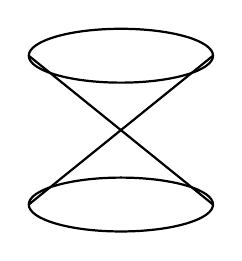
\begin{tikzpicture}[scale=0.9,line width=0.8pt]
  \draw (0,1.05) ellipse (1.30 and 0.38);
  \draw (0,-1.05) ellipse (1.30 and 0.38);
  \draw (-1.30,1.05) -- (1.30,-1.05);
  \draw (1.30,1.05) -- (-1.30,-1.05);
\end{tikzpicture}
\caption{$\mathbb{A}^3$ 中的\trCone{} $x^2+y^2=z^2$。（依原书手绘图重绘。）}\label{fig:traditional-cone}
\end{figure}

\textbf{9.3.Q.（练习：综合运用上面的若干概念）}\quad 证明：$\mathbb{P}(1,1,n)$ \trIsomorphic{}于 $n$ 次\trRationalNormalCurve{}上的\trProjective\trCone。
